\section{Background Work}\label{sec:background}
% (10 mins)

\begin{frame}[fragile, c]
    \frametitle{Bootstrapping: STLC and \HM{} type system}
    \begin{center}

      \uncover<+->{
        \begin{minipage}[h]{0.45\linewidth}
          \begin{flalign*}
            \lambda x. M
            &\begin{cases}
              \text{Abstract over computation}\\
              \text{Define functions}
            \end{cases}\\
            M N
            &\begin{cases}
              \text{Do the computation}\\
              \text{Use functions}
            \end{cases}
          \end{flalign*}
        \end{minipage}%
      }%
      \uncover<+->{
        \begin{minipage}[h]{0.45\linewidth}
          \begin{flalign*}
            \lambda x. M: {\color{red}\tau \rightarrow \tau'}
            &\begin{cases}
              x: {\color{red}\tau}\\
              M: {\color{red}\tau'}
            \end{cases}\\
            M N: {\color{red}\tau'}
            &\begin{cases}
              M: {\color{red}\tau \rightarrow \tau'}\\
              N: {\color{red}\tau}
            \end{cases}
          \end{flalign*}
        \end{minipage}
      }

    \end{center}
\end{frame}


% \begin{frame}[c]
%   \frametitle{Bootstrapping: STLC and \HM{} type system}
%   \begin{center}
%     \uncover<+->{
%       \begin{flalign*}
%         \lambda x. M
%         &\begin{cases}
%           \text{Abstract over computation}\\
%           \text{Define functions}
%         \end{cases}\\
%         M N
%         &\begin{cases}
%           \text{Do the computation}\\
%           \text{Use functions}
%         \end{cases}
%       \end{flalign*}
%     }
%     \uncover<+-> {
%       \begin{figure}[h]
%         \centering
%         % -> I
%         \begin{minipage}{0.5\textwidth}
%           \begin{prooftree}
%             \AxiomC{$\Gamma_{x}, x: \tau \vdash M : \tau'$} \RightLabel{[$\rightarrow$ I]}
%             \UnaryInfC{$\Gamma \vdash \lambda x. M : \tau \rightarrow \tau'$}
%           \end{prooftree}
%         \end{minipage}\hfill%
%         % -> E
%         \begin{minipage}{0.5\textwidth}
%           \begin{prooftree}
%             \AxiomC{$\Gamma \vdash M : \tau \rightarrow \tau'$}
%             \AxiomC{$\Gamma \vdash N : \tau$} \RightLabel{[$\rightarrow$ E]}
%             \BinaryInfC{$\Gamma \vdash M N : \tau'$}
%           \end{prooftree}
%         \end{minipage}
%       \end{figure}
%     }\vspace{1cm}
%     \uncover<+->{
%       Hindley-Milner (\HM{}) type system ensures sane programs
%     }
%   \end{center}
% \end{frame}

% \begin{frame}[c]
%   \frametitle{Bootstrapping: Simply Typed Lambda Calculus (STLC)}
%   \begin{center}
%     \fbox{Types and Typing Context}
%     \begin{flalign*}
%     t, u &\in \text{Type Variables}\\
%     \text{Types}\ \ \  \tau, \upsilon &::= t \mid \iota \mid \tau \rightarrow \tau\\
%     \text{Typing Scheme}\ \ \  \sigma &::= \tau \mid \forall t. \tau\\
%     \text{Typing Context}\ \ \ \Gamma &::= \epsilon \mid \Gamma, x:\sigma
%     \end{flalign*}
%     \fbox{Language}
%     \begin{flalign*}
%       \text{Expressions}\ \ \ M, N &::= x\\
%       &\mid \lambda x. M \mid M N\\
%       &\mid \Let{x}{M}{N}
%        \end{flalign*}
%      \end{center}
% \end{frame}

% \begin{frame}[c]
%   \frametitle{Bootstrapping: Hindley-Milner Type System}
%   \begin{center}
%   Hindley-Milner (\HM{}) type system\\
%   Type inferencing and Type checking:\\
%   \begin{itemize}
%   \item Algorithm $\M{}$\footfullcite{damas_principal_1982}\\
%   \item Algorithm $\W{}$\footfullcite{lee_proofs_1998}\\
% \end{itemize}
%   Type unification:\\
%   \begin{itemize}
%   \item Robinson's Algorithm $\Unf{}$\footfullcite{robinson_machine-oriented_1965}
% \end{itemize}
% \end{center}
% \end{frame}


% \begin{frame}
%   \frametitle{Bootstrapping: Typing Rules STLC}
%   \begin{center}
%     {\small
%     \begin{figure}[h]
%         % var
%         \begin{minipage}{.5\textwidth}
%           \begin{prooftree}
%             \AxiomC{$x: \sigma \in \Gamma$} \RightLabel{[VAR]}
%             \UnaryInfC{$\Gamma \vdash x : \sigma $}
%           \end{prooftree}
%         \end{minipage}\hfill%
%         % let
%         \begin{minipage}{.5\textwidth}
%           \begin{prooftree}
%             \AxiomC{$\Gamma \vdash M : \sigma$}
%             \AxiomC{$\Gamma_{x}, x: \sigma \vdash N: \tau$} \RightLabel{[LET]}
%             \BinaryInfC{$\Gamma \vdash (\Let{x}{M}{N}) : \tau$}
%           \end{prooftree}
%         \end{minipage}

%         % forall I
%         \begin{minipage}{0.5\textwidth}
%           \begin{prooftree}
%             \AxiomC{$\Gamma \vdash M : \sigma$}\RightLabel{[$\forall$ I]}
%             \AxiomC{$t \notin \texttt{fvs}(\Gamma)$}
%             \BinaryInfC{$\Gamma \vdash M : \forall t. \sigma$}
%           \end{prooftree}
%         \end{minipage}\hfill%
%         % forall E
%         \begin{minipage}{0.5\textwidth}
%           \begin{prooftree}
%             \AxiomC{$\Gamma \vdash M : \sigma$}
%             \AxiomC{$(\sigma' \sqsubseteq \sigma)$}\RightLabel{[$\forall$ E]}
%             \BinaryInfC{$\Gamma \vdash M : \sigma'$}
%           \end{prooftree}
%         \end{minipage}

%         % -> I
%         \begin{minipage}{0.5\textwidth}
%           \begin{prooftree}
%             \AxiomC{$\Gamma_{x}, x: \tau \vdash M : \tau'$} \RightLabel{[$\rightarrow$ I]}
%             \UnaryInfC{$\Gamma \vdash \lambda x. M : \tau \rightarrow \tau'$}
%           \end{prooftree}
%         \end{minipage}\hfill%
%         % -> E
%         \begin{minipage}{0.5\textwidth}
%           \begin{prooftree}
%             \AxiomC{$\Gamma \vdash M : \tau \rightarrow \tau'$}
%             \AxiomC{$\Gamma \vdash N : \tau$} \RightLabel{[$\rightarrow$ E]}
%             \BinaryInfC{$\Gamma \vdash M N : \tau'$}
%           \end{prooftree}
%         \end{minipage}
%     \end{figure}
%     }
%   \end{center}
% \end{frame}

% \begin{frame}
%   \frametitle{Bootstrapping: Algorithm $\M{}$}
%   \begin{center}
%   \begin{figure}[h]
%     \centering
%     {\small
%       \fbox{$\M(\Gamma \vdash M:\tau) = S$}\\
%       % VAR
%       \begin{minipage}{0.45\linewidth}
%         \begin{flalign*}
%             \M(\Gamma \vdash &x:\tau)  = \mathcal{U}(\tau, [\vec{u}/\vec{t}]\upsilon)\\
%             &\text{where\qquad}\  \forall \vec{t}. \upsilon = \Gamma(x)
%         \end{flalign*}
%       \end{minipage}\hfill%
%       % \x. M
%       \begin{minipage}{0.50\linewidth}
%         \begin{flalign*}
%           \M(\Gamma \vdash &\lambda x. M:\tau) = S  \circ S' \\
%             \text{where\qquad}\ S  &= \mathcal{U}(\tau, u_1 \rightarrow u_2)\\
%             S'  &= \M(S \Gamma, x: S  u_1 \vdash M : S u_2)
%           \end{flalign*}
%       \end{minipage}

%       % M N
%       \begin{minipage}{0.45\linewidth}
%         \begin{flalign*}
%           \M(\Gamma \vdash &M N:\tau)  = S  \circ S' \\
%           \text{where\qquad}\ S  &= \M(\Gamma \vdash M: u \rightarrow \tau)\\
%           S'  &= \M(S  \Gamma \vdash N: S u)
%         \end{flalign*}
%       \end{minipage}\hfill%
%       % let x = M in N
%       \begin{minipage}{0.50\linewidth}
%         \begin{flalign*}
%           \M(\Gamma \vdash (&\Let{x}{M}{N}):\tau) = S  \circ S' \\
%           \text{where\qquad}\ S  &= \M(\Gamma \vdash M: u)\\
%                               \sigma &= \texttt{Gen}(S \Gamma, S u)\\
%                               S' &= \M(S \Gamma, x:\sigma \vdash N:\tau)\\
%         \end{flalign*}
%       \end{minipage}

%       % \fbox{Auxiliary Definitions}

%       % \begin{minipage}{0.45\linewidth}
%       %   \begin{flalign*}
%       %     \texttt{Gen}(\Gamma, \tau) &= \forall \vec{t}. \tau\\
%       %     \text{where\qquad}\ \vec{t} &= \texttt{fvs}(\tau)\backslash\texttt{fvs}(\Gamma)
%       %   \end{flalign*}
%       % \end{minipage}%
%       % \begin{minipage}{0.45\linewidth}
%       %   \begin{flalign*}
%       %     \texttt{fvs}(t) &= \{t\}\\
%       %     \texttt{fvs}(\forall \vec{t}. \tau) &= \texttt{fvs}(\tau) \backslash \vec{t}\\
%       %     \texttt{fvs}(\Gamma) &= \bigcup_{\forall (x:\sigma) \in \Gamma} \texttt{fvs}(\sigma)
%       %   \end{flalign*}
%       % \end{minipage}

%     }
%   \label{fig:hm-algo-m}
% \end{figure}
% \end{center}
% \end{frame}


\begin{frame}[c]
  \frametitle{Bootstrapping: Curry-Howard Correspondence}
  \begin{center}
      \text{\HM{} type system} $\equiv$ \text{Second Order Intuitionistic Propositional Logic}
    \begin{itemize}
    \item Types are Propostions
    \item Programs are Proofs
    \end{itemize}

    \begin{figure}[h]
      \centering
      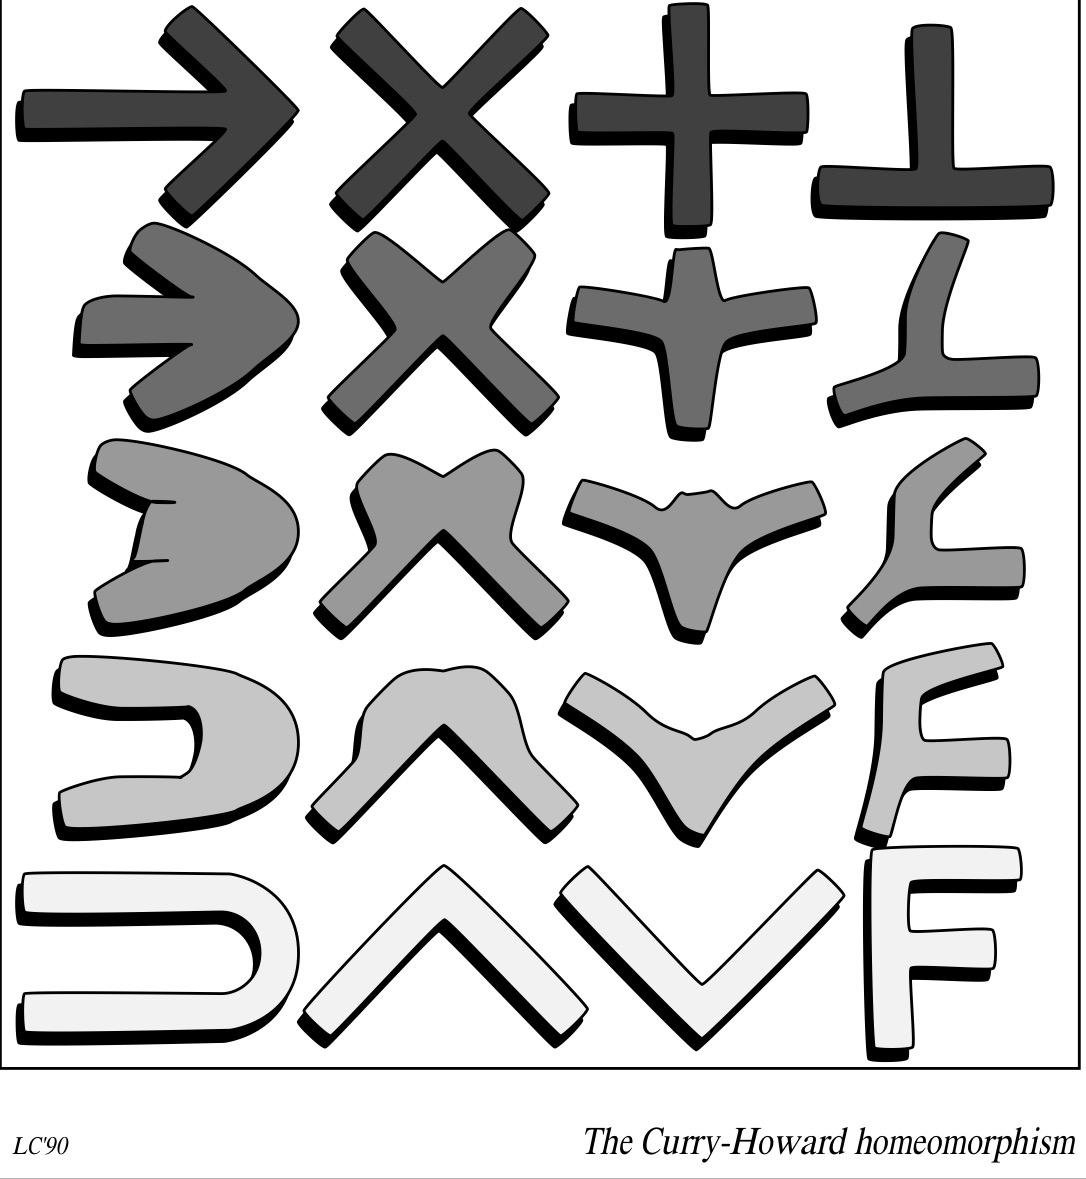
\includegraphics[scale=0.1]{defense-slides/cardelli-hc-corr.jpg}

      {{\tiny Source: \url{http://lucacardelli.name/Artifacts/Drawings/CurryHoward/CurryHoward.pdf}}}
    \end{figure}
\end{center}
\end{frame}

\begin{frame}[c]
  \frametitle{Bootstrapping: S O Intuitionistic Propositional Logic}
  \begin{center}
    \uncover<2->{{\LARGE \color{red}Propositions are truth values not resources}}\\
    \uncover<1->{
        \fbox{Language}
        \begin{flalign*}
          \text{Propositions and Connectives}\quad A, B, C &::= x \mid A \supset B \mid \forall x. B \mid A \vee B \mid A \wedge B \\
          \text{Context}\quad \Gamma,\Delta &::= \epsilon \mid \Gamma, A
        \end{flalign*}
        \fbox{Implicit Structural Rules}

        \begin{tabular}[h]{c c c}
          $A, B \vdash A$ &  $A, B \vdash B$   & Weakening \\

          \multicolumn{2}{c}{$A \vdash A \wedge A$} & Contraction \\

          \multicolumn{2}{c}{$A, B \vdash B, A$} & Exchange
        \end{tabular}
      }
  \end{center}
\end{frame}

\begin{frame}[c]
  \frametitle{Bootstrapping: Substructural Logic}
  \begin{center}
{\small     \begin{tabular}[h]{c c c c}
      System                                                                                 &  Who             & Year         & Control\\ \hline\hline
      Revelance Logic\footnote[frame]{{\tiny \fullcite{orlov_relevence_1928}}}               & Orlev            & 1928         & [WKN]\\
      Lambek Logic\footnote[frame]{{\tiny \fullcite{lambek_mathematics_1958}}}               & Lambek           & 1958         & [EXCH]\\
      Affine Logic\footnote[frame]{{\tiny \fullcite{grishin_affine_1974}}}                         & Grishin          & 1974         & [CTR] \\
      Linear Logic\footnote[frame]{{\tiny \fullcite{girard_linear_1987}}}                    & Girard           & 1987         & [WKN] [CTR]\\
      \color{red}{Logic of Bunched Implications}\footnote[frame]{{\tiny \fullcite{ohearn_logic_1999}}}    & \color{red}{O'Hearn and Pym}  & \color{red}{1999} & \color{red}{[WKN] [CTR]}\\
      Separation Logic \footnote[frame]{{\tiny \fullcite{reynolds_separation_2002}}}         & Reynolds         & 2002         & [WKN] [CTR] \\
      \vdots                                                                       & \vdots              & \vdots          & \vdots
    \end{tabular}
}  \end{center}
\end{frame}

\begin{frame}
  \frametitle{Bootstrapping: Logic of \BI{}}
  \begin{center}
    Coffee Shop

    1 cup coffee costs \$2

    \uncover<1->{
      \begin{tabular}[c]{c c c c c}
        \raisebox{-0.4\height}{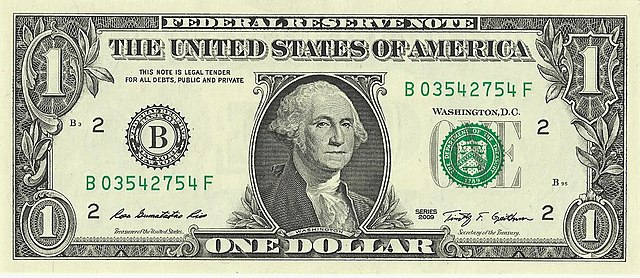
\includegraphics[scale=0.15]{defense-slides/one_usd}}
        & {\LARGE $,$}
        & \raisebox{-0.4\height}{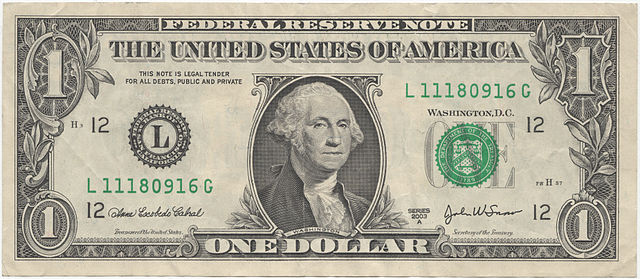
\includegraphics[scale=0.151]{defense-slides/one_usd_2}}
        & {\LARGE $\vdash$}
        & \raisebox{-0.4\height}{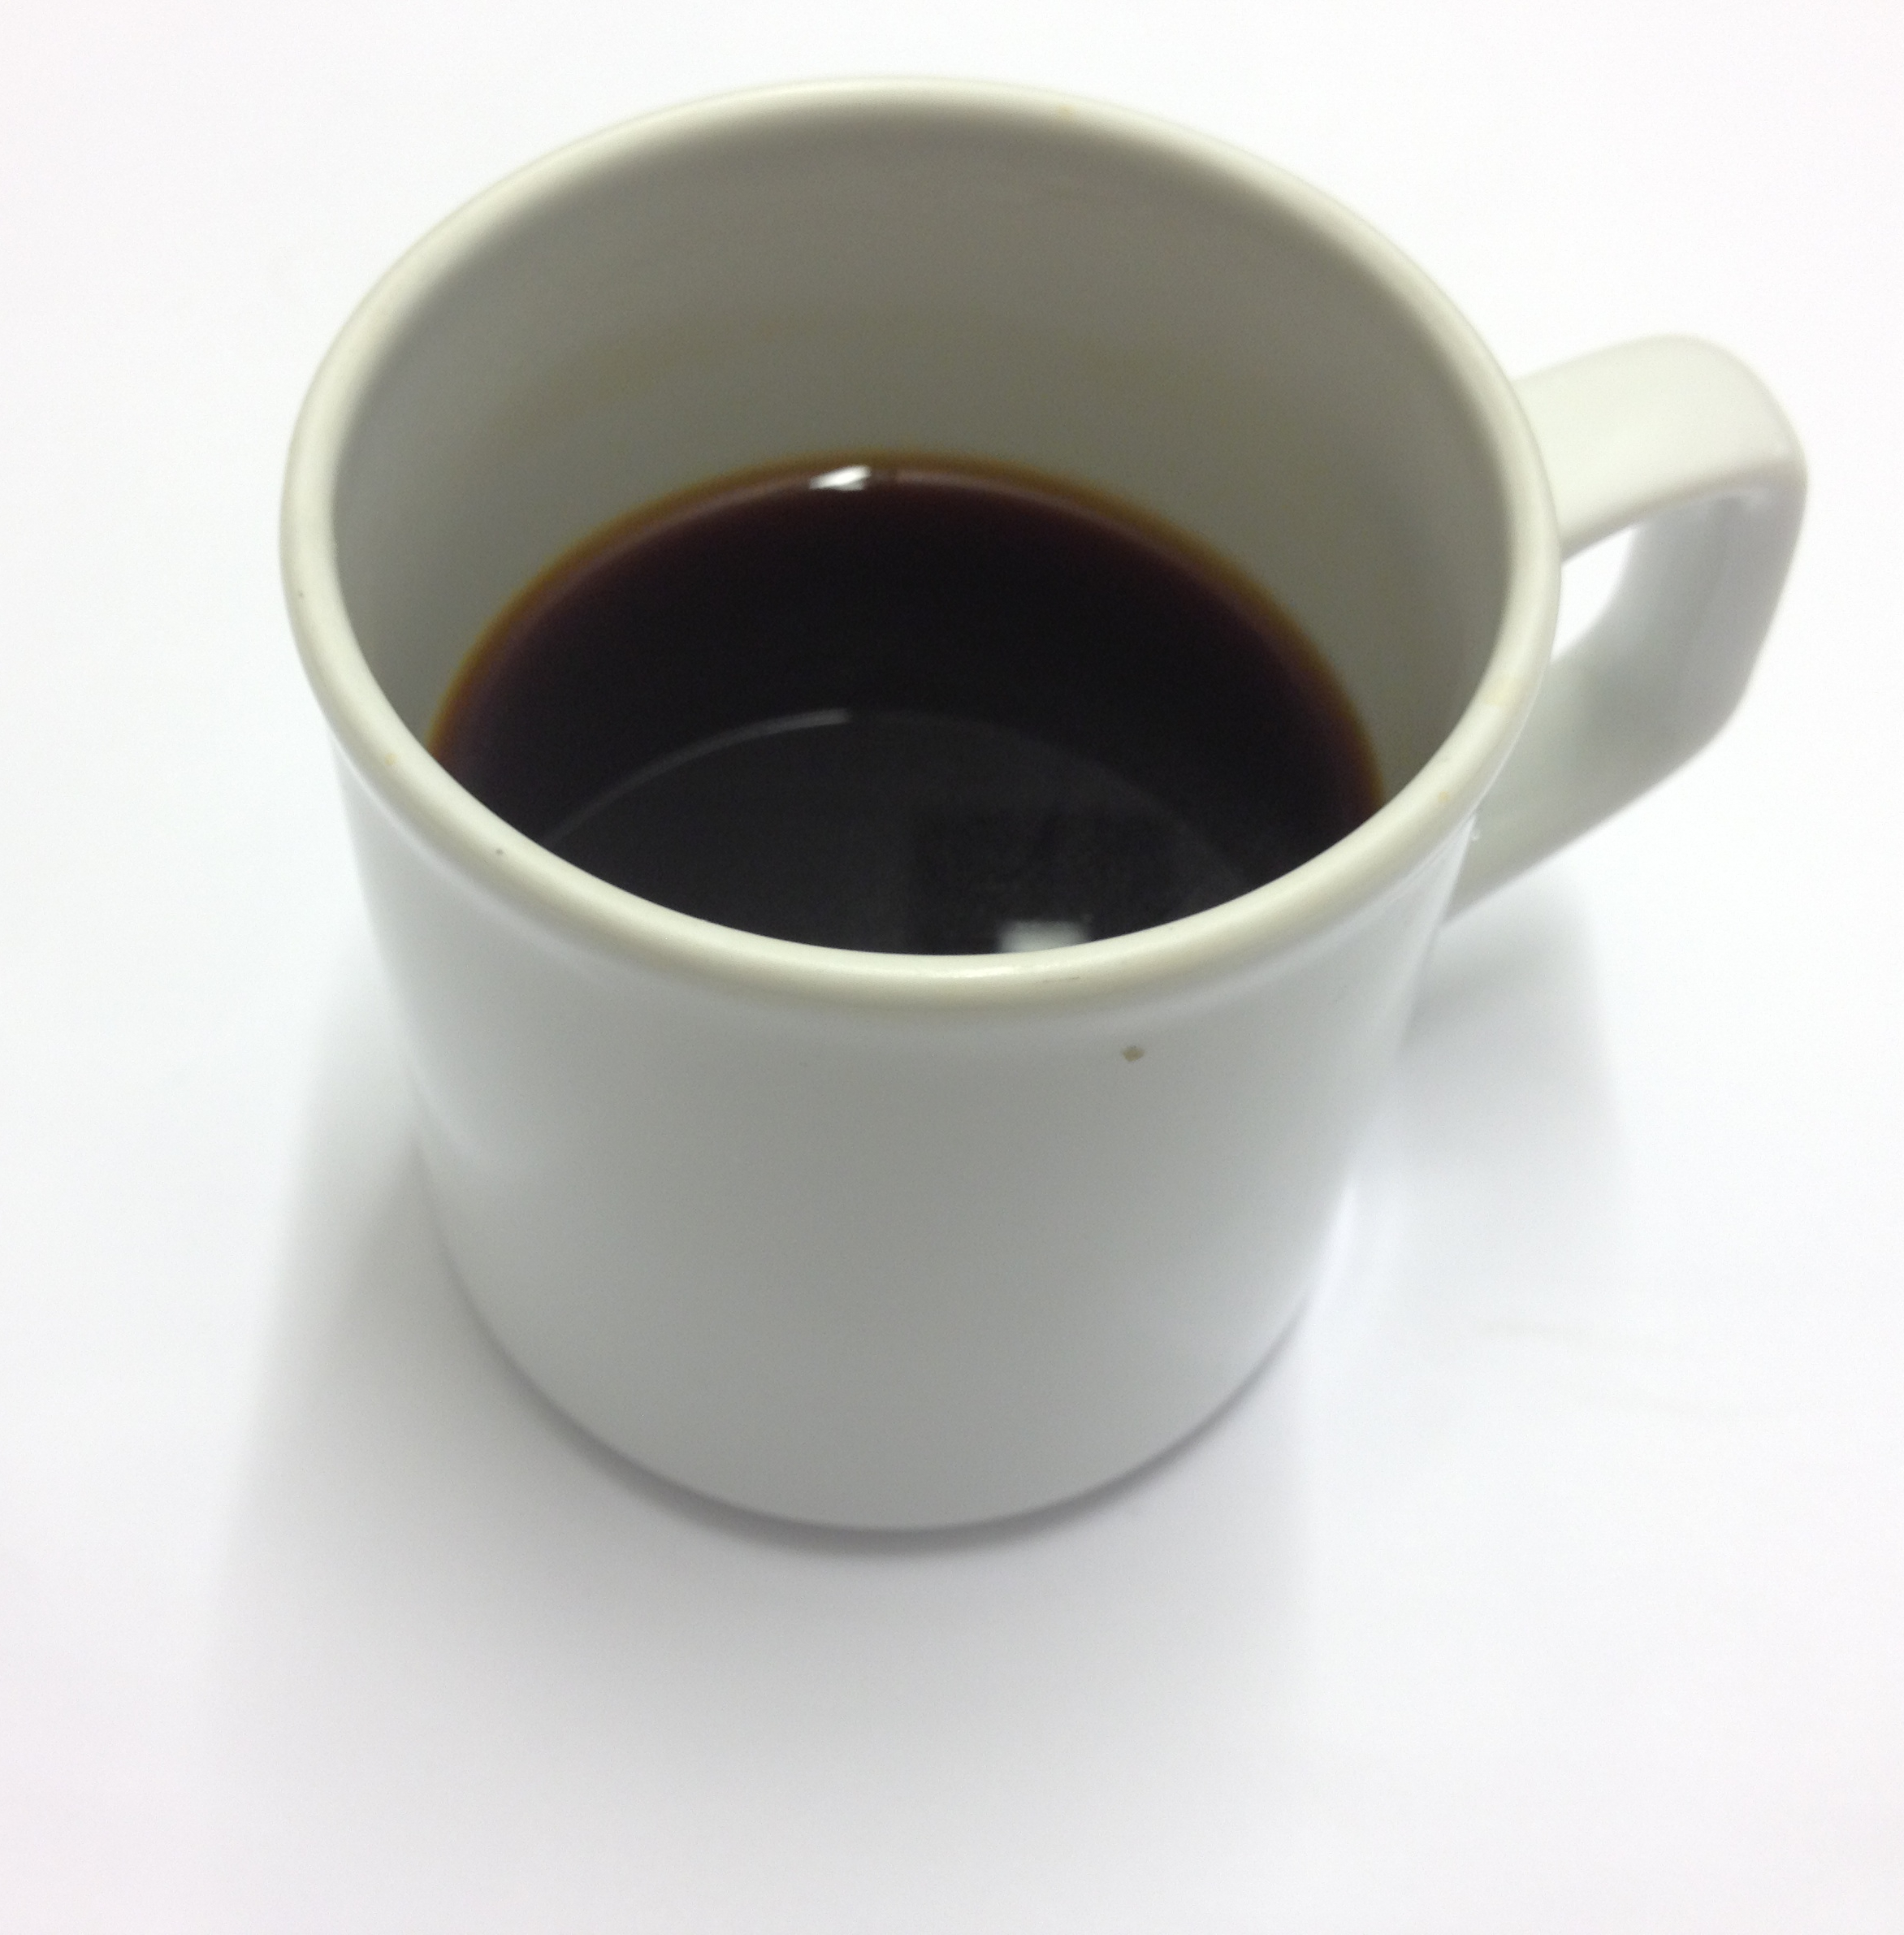
\includegraphics[scale=0.03]{defense-slides/coffee_cup}}
      \end{tabular}
    }
    \uncover<2->{
      \begin{tabular}[c]{c c c c c}
        \raisebox{-0.4\height}{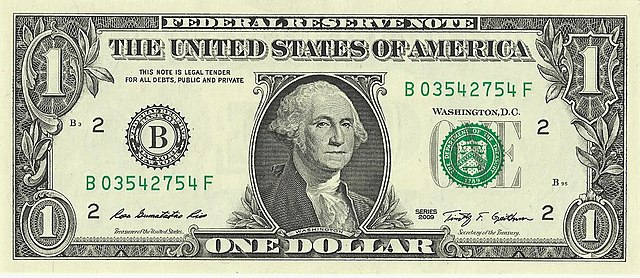
\includegraphics[scale=0.15]{defense-slides/one_usd}}
        & {\LARGE $,$}
        & \raisebox{-0.4\height}{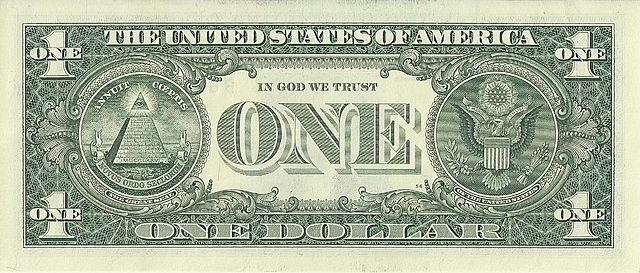
\includegraphics[scale=0.2]{defense-slides/one_usd_rev}}
        & {\LARGE $\not\vdash$}
        & \raisebox{-0.4\height}{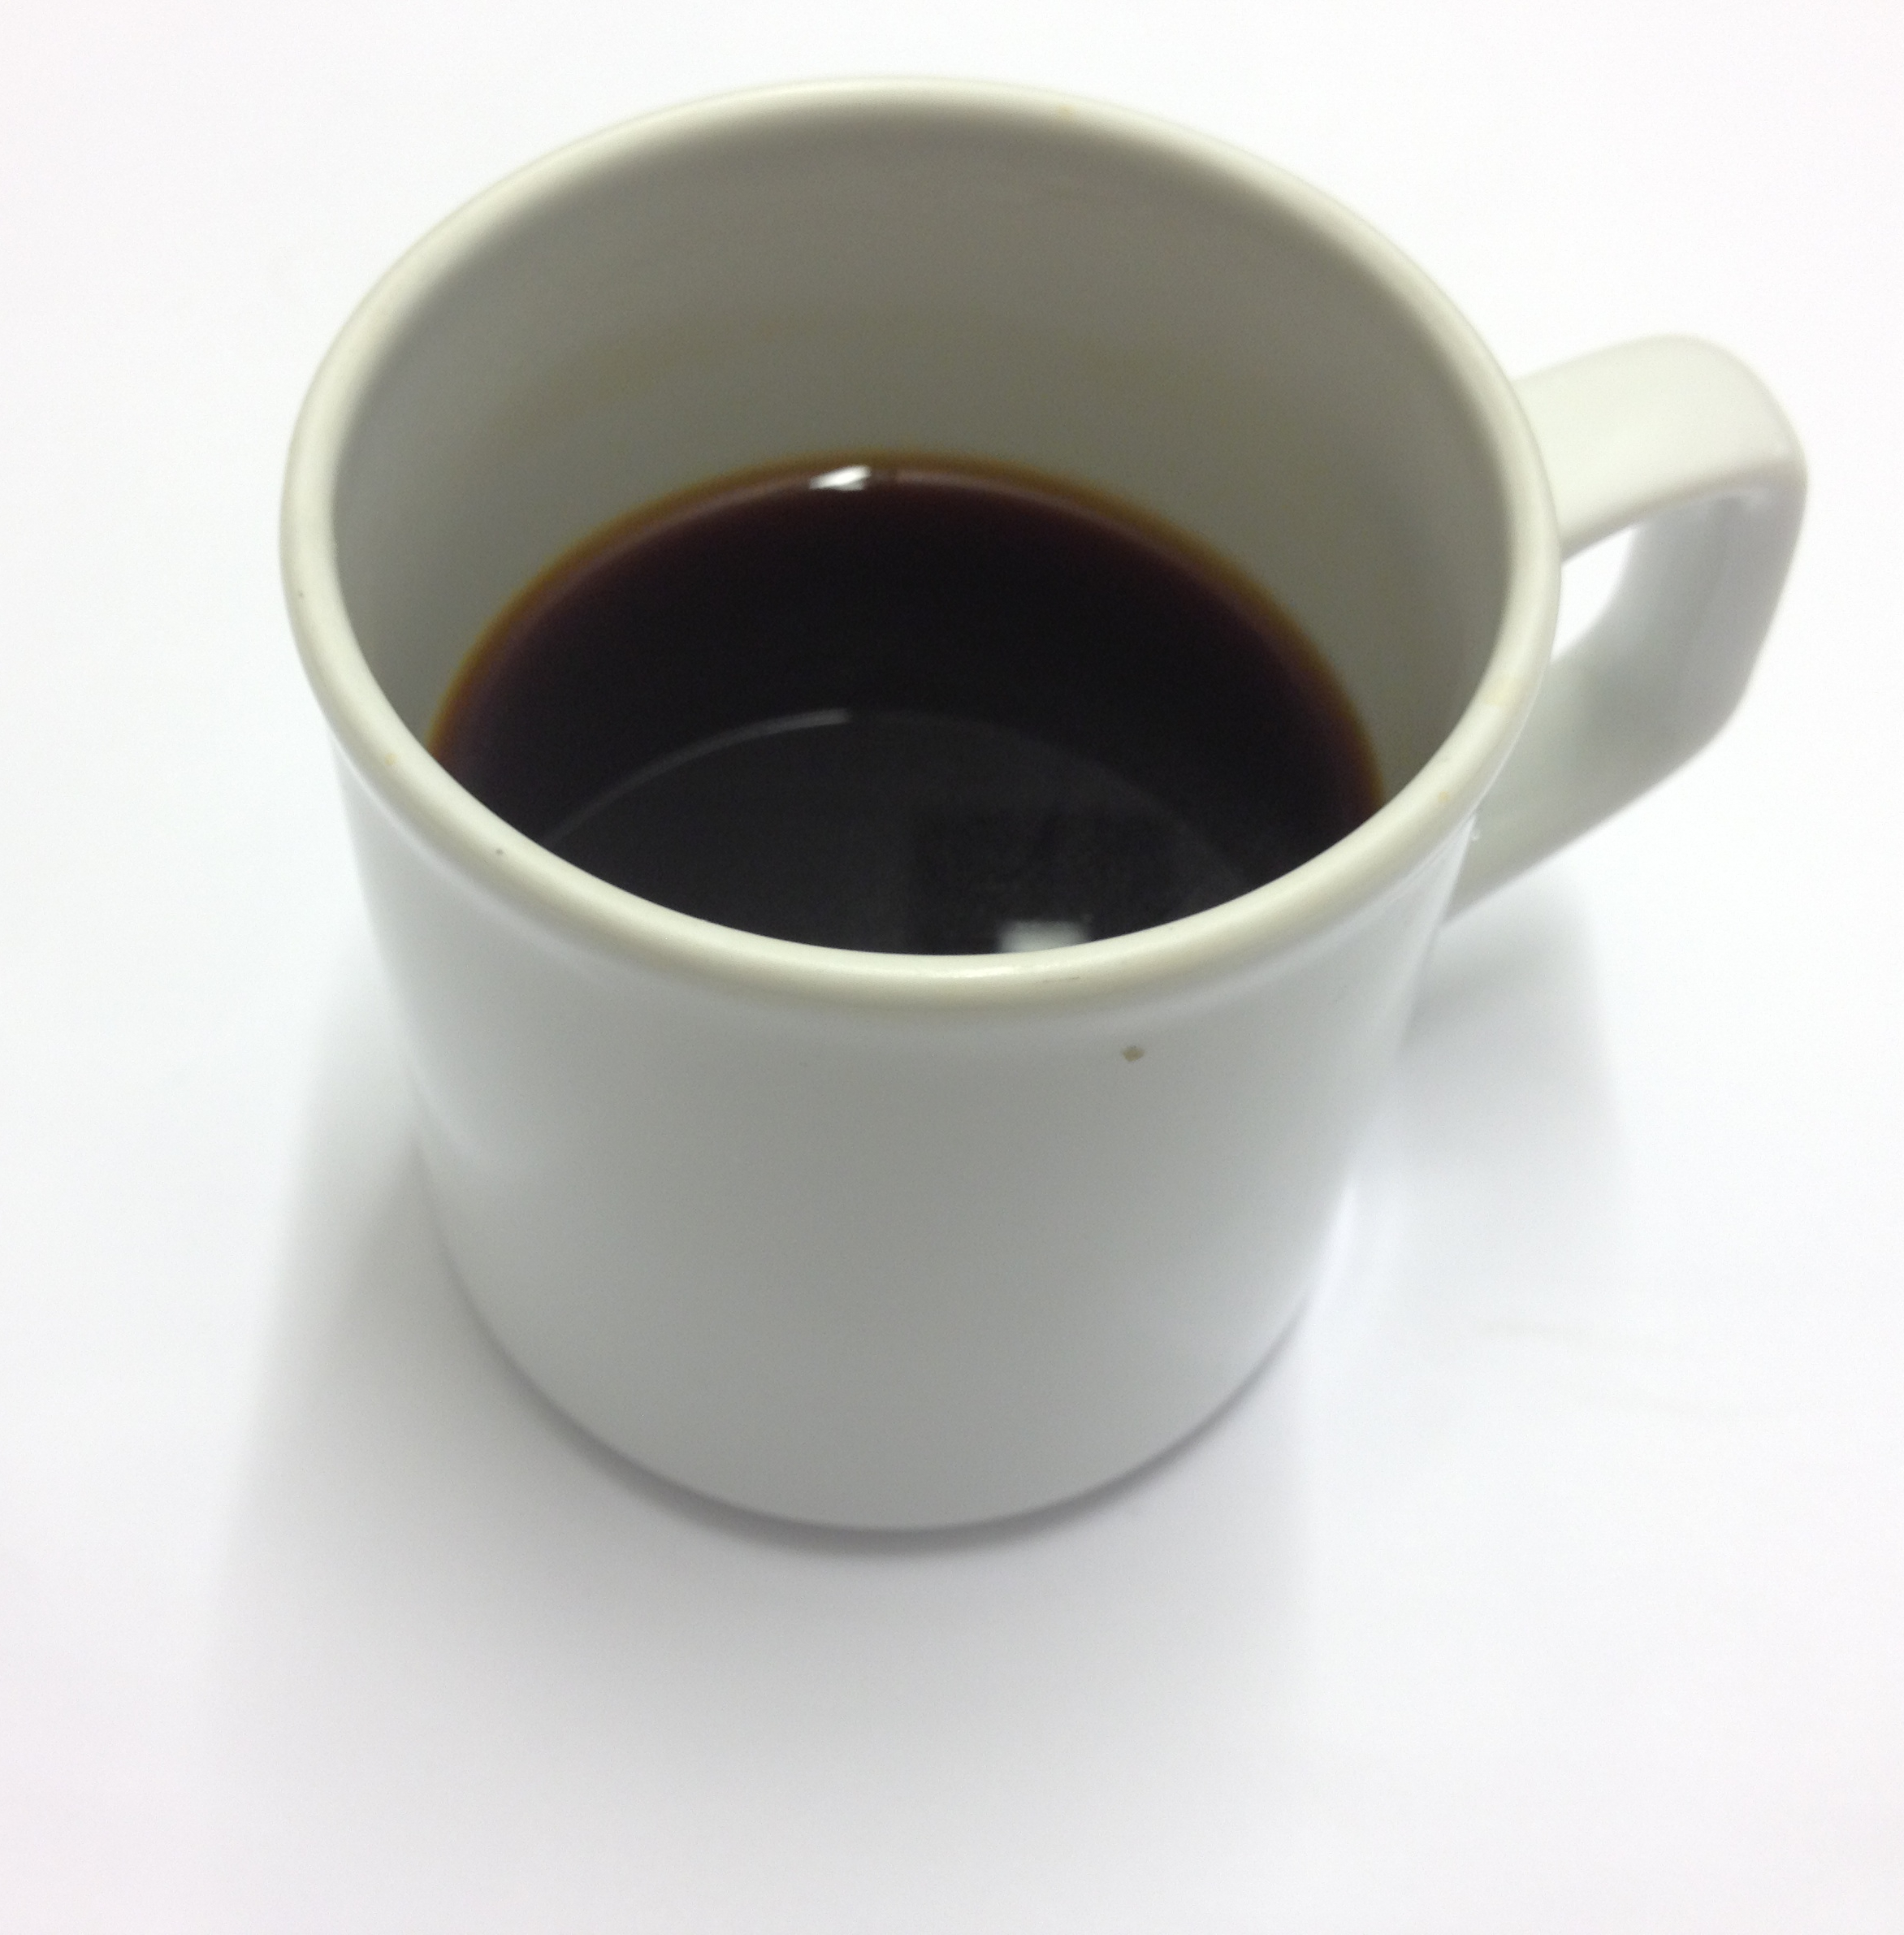
\includegraphics[scale=0.03]{defense-slides/coffee_cup}}
      \end{tabular}

      {\color{red}two separate} dollar bills necessary
    }
  \end{center}
\end{frame}

\begin{frame}[c]
  \frametitle{Bootstrapping: Logic of \BI{}}
  \begin{center}
    \begin{itemize}

    \item<1-> Conjunction ($\wedge$) split into two flavors
      \begin{center}
      \begin{tabular}[c]{c l}
      $A \otimes B$& A is separate from B\\
      $A \with B$&  A is a different view of B or A shares with B
      \end{tabular}
    \end{center}
    \item<2-> \BI{} contexts sensitive to different conjunction
      \begin{center}
        \begin{minipage}[h]{0.5\linewidth}
          $A, B \vdash A \otimes B$
        \end{minipage}%
        \begin{minipage}[h]{0.5\linewidth}
          $A; B \vdash A \with B$
        \end{minipage}
    \end{center}
    \item<3-> Contexts form trees, called bunches
      \begin{center}
        \begin{figure}[h]\centering
      \begin{minipage}{0.5\linewidth}\centering
        \tikzset{every tree node/.style={minimum width=2em},
          blank/.style={draw=none},
          edge from parent/.style=
          {draw,edge from parent path={(\tikzparentnode) -- (\tikzchildnode)}},
          level distance=1.5cm}
        \begin{tikzpicture}
          \Tree
          [.,
          [.;
          [.A ]
          [.B ]
          ]
          [.C ]
          ]
        \end{tikzpicture}
        \caption*{$(A;B),C$}
      \end{minipage}%
      \begin{minipage}{0.5\linewidth}\centering
        \tikzset{every tree node/.style={minimum width=2em},
          blank/.style={draw=none},
          edge from parent/.style=
          {draw,edge from parent path={(\tikzparentnode) -- (\tikzchildnode)}},
          level distance=1.5cm}
        \begin{tikzpicture}
          \Tree
          [.;
          [.A ]
          [.,
          [.C ]
          [.B ]
          ]
          ]
        \end{tikzpicture}
        \caption*{$A;(B,C)$}
      \end{minipage}
    \end{figure}

    \end{center}

\end{itemize}
\end{center}
\end{frame}

\begin{frame}[c]
  \frametitle{Bootstrapping: Logic of \BI{}}
  \begin{center}
  Context connectives guide structural rules

  \begin{itemize}
  \item Contraction
    \begin{center}
      $A \vdash A;A$\\
      $A \not\vdash A,A$
    \end{center}

  \item Weakening
    \begin{center}
      $A;A \vdash A$ \qquad $A;B \vdash B$ \qquad $A;B \vdash A$\\
      $A,B \not\vdash A$ \qquad $A,B \not\vdash B$
    \end{center}
  \end{itemize}
\end{center}
\end{frame}

\begin{frame}
  \frametitle{Bootstrapping: Logic of \BI{}}
  \begin{center}
    Coffee Shop (Revisited)

    1 cup coffee costs \$2 \qquad  1 cookie costs \$1
    \begin{tabular}[c]{c c c c c}
        \raisebox{-0.4\height}{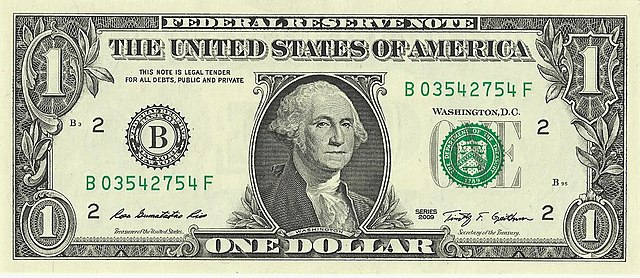
\includegraphics[scale=0.12]{defense-slides/one_usd}}
        & {\LARGE $\vdash$}
        & \raisebox{-0.4\height}{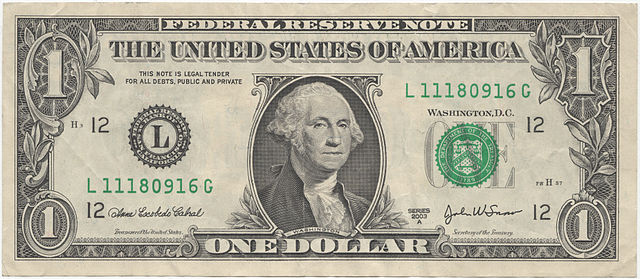
\includegraphics[scale=0.121]{defense-slides/one_usd_2}}
        & {\LARGE $\sepimp$}
        & \raisebox{-0.4\height}{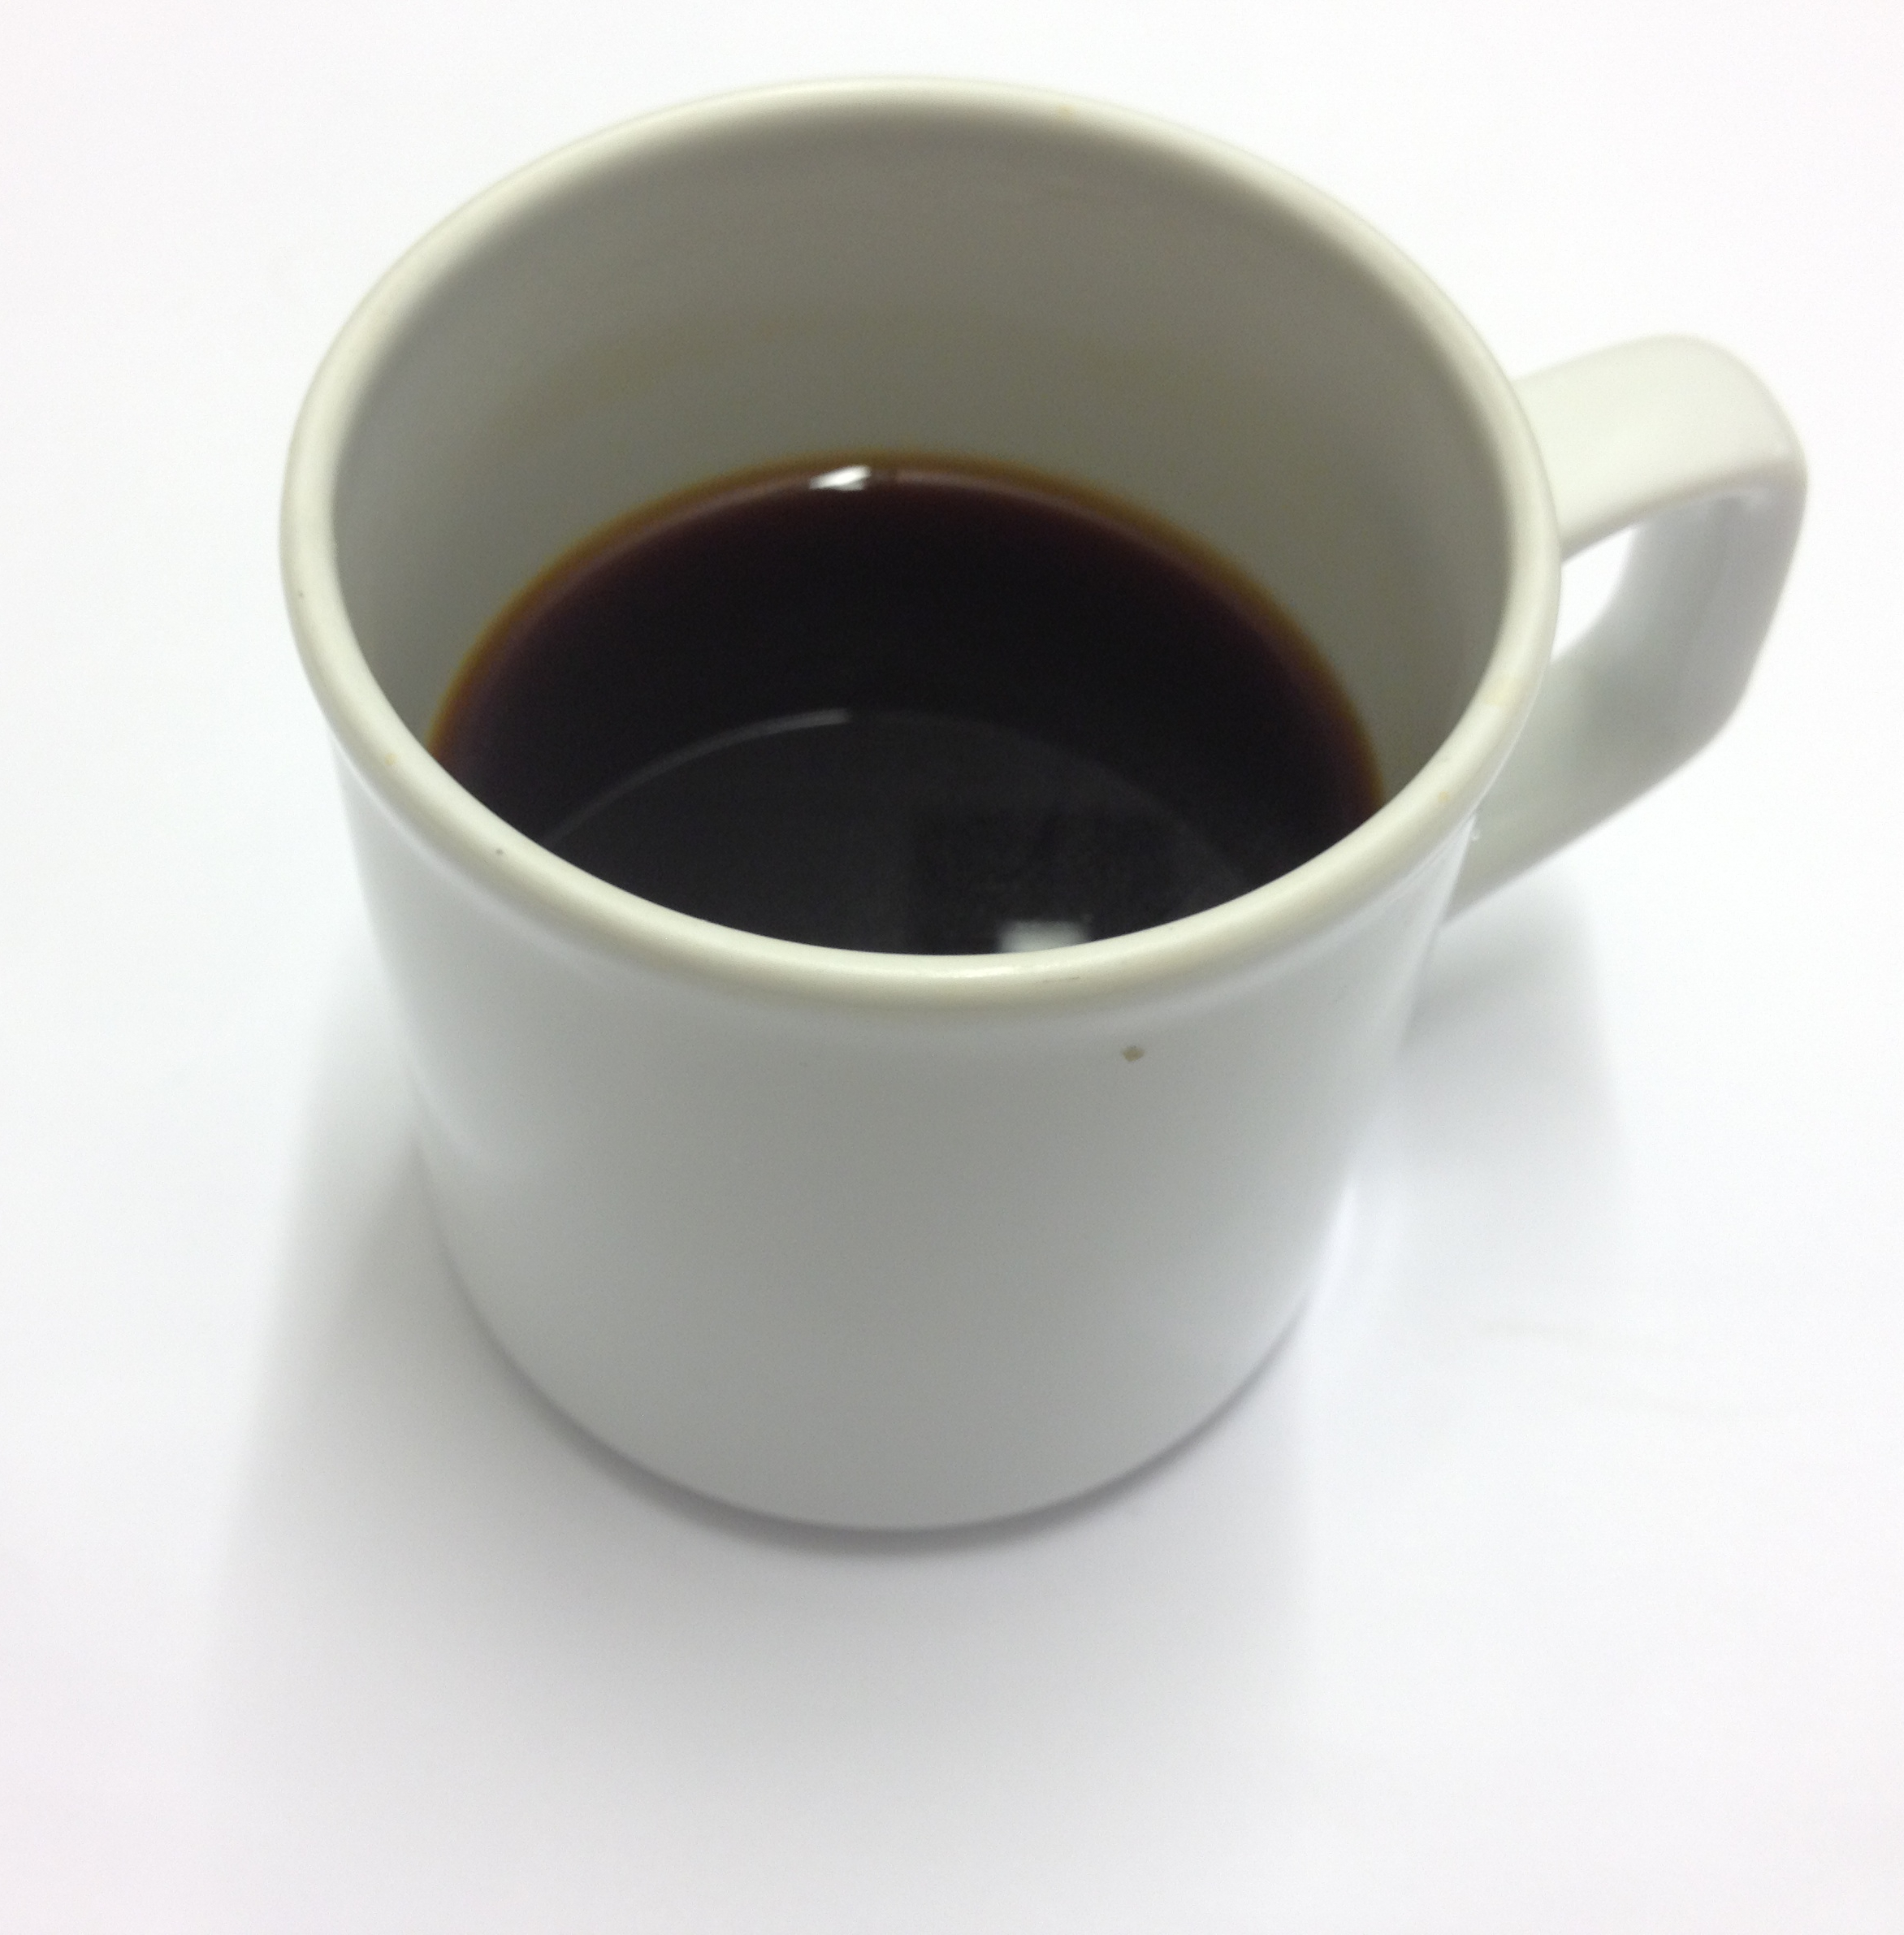
\includegraphics[scale=0.025]{defense-slides/coffee_cup}}
      \end{tabular}

      \begin{tabular}[c]{c c c c c}
        \raisebox{-0.4\height}{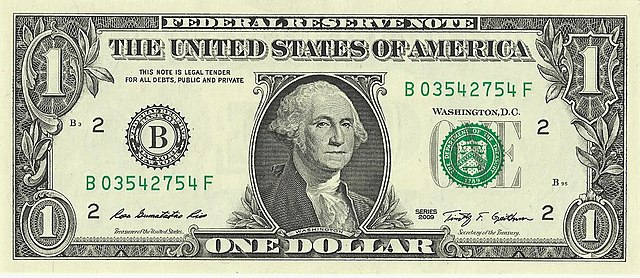
\includegraphics[scale=0.12]{defense-slides/one_usd}}
        & {\LARGE $\vdash$}
        & \raisebox{-0.4\height}{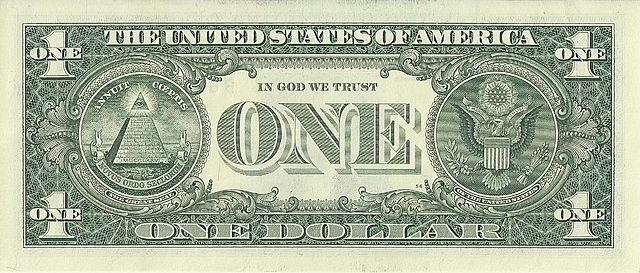
\includegraphics[scale=0.16]{defense-slides/one_usd_rev}}
        & {\LARGE $\shimp$}
        & \raisebox{-0.4\height}{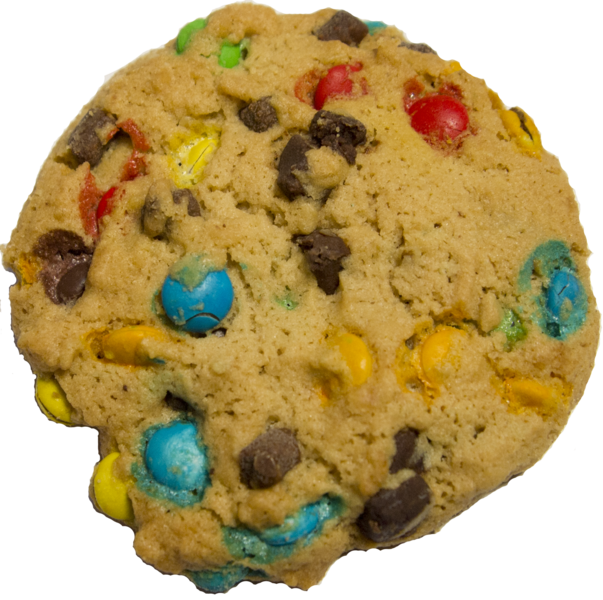
\includegraphics[scale=0.25]{defense-slides/cookie}}
      \end{tabular}

      \begin{tabular}[c]{c c c c c}
        \raisebox{-0.4\height}{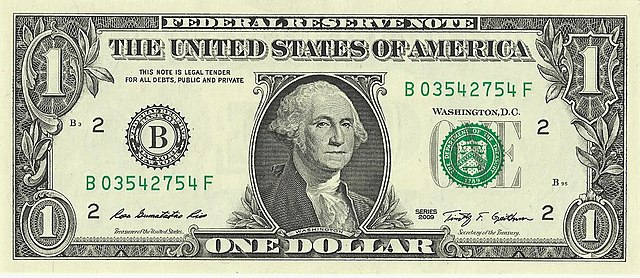
\includegraphics[scale=0.12]{defense-slides/one_usd}}
        & {\LARGE $\not\vdash$}
        & \raisebox{-0.4\height}{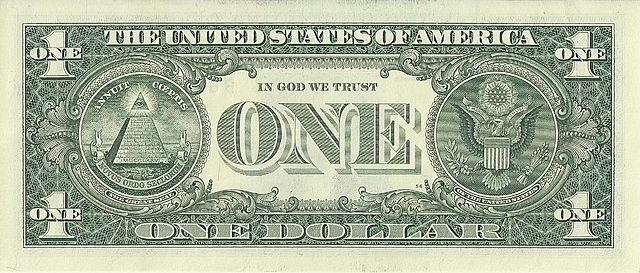
\includegraphics[scale=0.17]{defense-slides/one_usd_rev}}
        & {\LARGE $\shimp$}
        & \raisebox{-0.4\height}{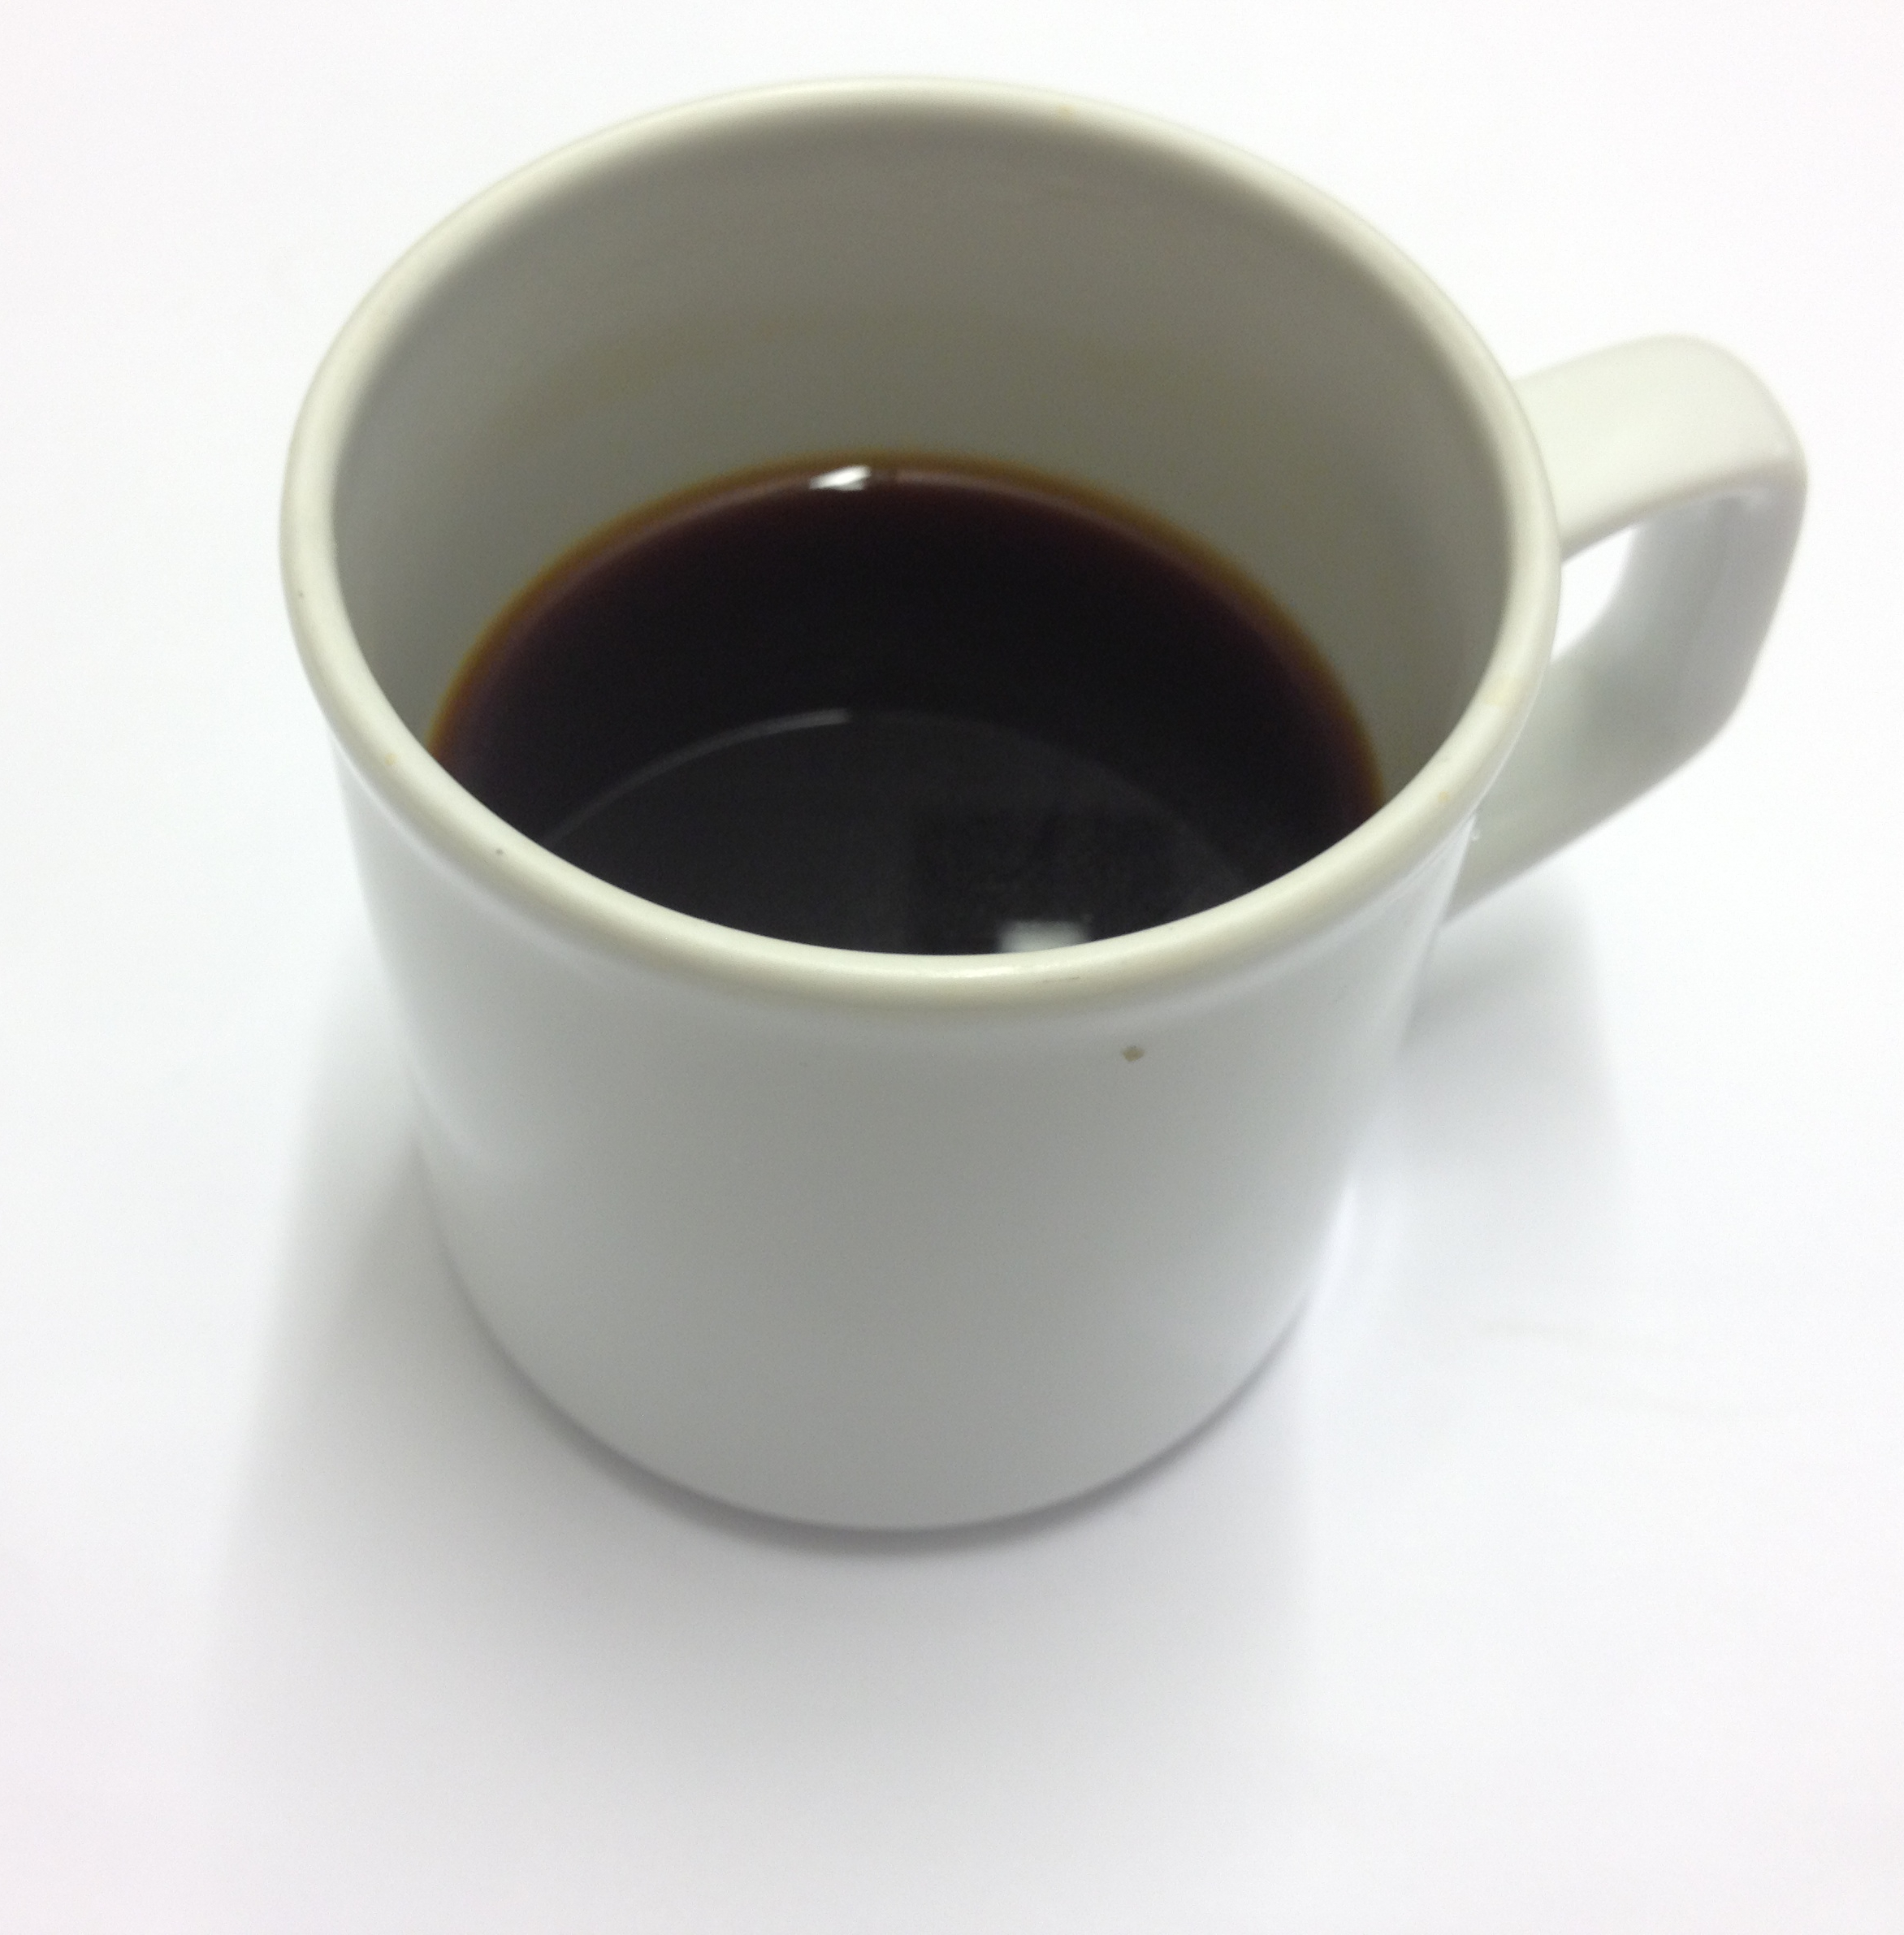
\includegraphics[scale=0.025]{defense-slides/coffee_cup}}
      \end{tabular}

  \end{center}
\end{frame}

\begin{frame}[c]
  \frametitle{Bootstrapping: Logic of \BI{}}
  \begin{center}
    Implications get corresponding flavors

    $A \otimes B \vdash C\ \text{iff}\ A \vdash B \sepimp C$

    $A \with B \vdash C\ \text{iff}\ A \vdash B \shimp C$
  \end{center}
\end{frame}


%%% Local Variables:
%%% mode: latex
%%% TeX-master: "defense-slides"
%%% End:
